\documentclass[12pt, a4paper]{article}

% ------------------------------ font
\usepackage{times} %pdflatex
% \usepackage{luatexja}
% \usepackage{luatexja-fontspec}

% \setmainfont{Times New Roman}
% \setmainjfont[BoldFont=IPAexGothic]{IPAexMincho}

% ------------------------------ math
\usepackage{amsmath,amssymb}
\usepackage{siunitx}

% ------------------------------ author & natbib
\usepackage{authblk}
\usepackage[semicolon]{natbib}
\bibliographystyle{agsm}

% ------------------------------ appendix
\usepackage[title]{appendix}

% ------------------------------ tables
\usepackage{here}
\usepackage{longtable, booktabs, array}
\usepackage{threeparttable, threeparttablex, multirow}
% \newcolumntype{d}{S[input-symbols = ()]}

% ------------------------------- figures
\usepackage[labelfont=bf, labelsep=period, justification=justified]{caption}
\usepackage{graphics, graphicx}
\makeatletter
\def\maxwidth{\ifdim\Gin@nat@width>\linewidth\linewidth\else\Gin@nat@width\fi}
\def\maxheight{\ifdim\Gin@nat@height>\textheight\textheight\else\Gin@nat@height\fi}
\makeatother
% Scale images if necessary, so that they will not overflow the page
% margins by default, and it is still possible to overwrite the defaults
% using explicit options in \includegraphics[width, height, ...]{}
\setkeys{Gin}{width=\maxwidth,height=\maxheight,keepaspectratio}

% ------------------------------ page settings
\usepackage[left=3cm,right=3cm,top=3cm,bottom=3cm]{geometry}
\usepackage{setspace}
\renewcommand{\baselinestretch}{2}
\providecommand{\tightlist}{%
  \setlength{\itemsep}{0pt}\setlength{\parskip}{0pt}}

% ------------------------------ hyperlink
\usepackage[hidelinks]{hyperref}

% ------------------------------ other packages
\usepackage{booktabs}
\usepackage{siunitx}

  \newcolumntype{d}{S[
    input-open-uncertainty=,
    input-close-uncertainty=,
    parse-numbers = false,
    table-align-text-pre=false,
    table-align-text-post=false
  ]}
  

% ------------------------------ paper information
\title{Only You:
Field Experiment Using Text Messages to Prevent Free-riding in the Japan Marrow Donor Program\thanks{We would like to thank the Japan Marrow Donor Program Office for managing the field experiment and providing us with the data. This study was conducted with the approval of the institutional review board of the Graduate School of Economics, Osaka University (approval number: R030305-2) and the Japan Marrow Donor Program (approval number: JMDP2021-04). Declarations of interest: none. Funding: This work was supported by the Japan Society for the Promotion of Science {[}grant number 20H05632{]} and the Ministry of Health, Labour and Welfare {[}grant number 19FF1001{]}.}}
\author{}
\date{}

\makeatletter
\renewcommand*{\@fnsymbol}[1]{\ifcase#1\or*\else\@arabic{\numexpr#1-1\relax}\fi}
\makeatother

\begin{document}
\begin{spacing}{1}
  \maketitle
    \clearpage
  \begin{abstract}
  Approximately half of the patients registered with the Japan Marrow Donor Program (JMDP) receive allogeneic hematopoietic stem cell transplantation from JMDP donors. This is because much of transplant coordination is interrupted before the confirmatory typing stage owing to donor-related reasons. A field experiment was conducted in collaboration with JMDP to verify the effects of providing information to increase the probability of donors reaching confirmatory typing (donor availability from whom physicians can choose the optimal one for transplantation). We found that providing information about the low number of compatible donors per patient increased the probability of donors reaching confirmatory typing by 14\%. Specifically, this information increased the probability of young male donors, who have better transplant outcomes, reaching the confirmatory typing by 28\% through increasing their willingness to donate.
  \vskip\baselineskip
  \noindent
  \textit{Keywords}: field experiment, free-riding, information provision, Japan Marrow Donor Program, present bias, text message
  \vskip\baselineskip
  \noindent
  \textit{JEL classification}: D64, D90, H41, I11
  \end{abstract}
  \end{spacing}



\setcounter{footnote}{0}
\clearpage

\hypertarget{intro}{%
\section{Introduction}\label{intro}}

Allogeneic hematopoietic stem cell transplantation (HSCT) is a treatment with the lowest relapse rates for leukemia and other blood diseases. In this treatment, (1) anticancer drugs and radiation kill tumor cells, and (2) healthy hematopoietic stem cells donated by others are transplanted. Transplantation requires that the donor's white blood cell type, known as human leukocyte antigen (HLA), fully or partially matches the patient's HLA. While the probability of a full match between two randomly selected unrelated individuals is below 1\%, siblings have the highest probability of a full match at approximately 30\%.

If no match exists among relatives, patients must seek an unrelated donor.\footnote{When HLA-identical or partially matched unrelated donors are unavailable, several alternative options exist. The first option is haploidentical stem cell transplantation, in which stem cells are transplanted from a close relative with semi-matched HLA. The second option is cord blood transplantation, in which stem cells are transplanted from the umbilical cord or placenta. The HLA requirements for these transplants are weaker than those for bone marrow (or peripheral blood) transplants between unrelated individuals. Notably, in Japan, bone marrow (or peripheral blood) transplants between unrelated individuals accounted for 20\% of all transplants performed in FY2021 \citep{JapaneseDataCenterf2022}.} Patients in Japan typically seek unrelated donors through the Japan Marrow Donor Program (JMDP). However, it takes a long time to confirm the donor's intention and ensure the safety of the transplant when coordinating through the JMDP. According to \citet{Hirakawa2018}, the median time required for transplantation through JMDP is 146 days (approximately five months), and only 60\% of registered patients receive transplants from JMDP-unrelated donors. Therefore, shortening the time to transplantation and increasing the transplantation rate among registered patients is crucial.

To increase transplantation rates, one possible intervention involves increasing the number of donors available for physicians to select the optimal match for transplantation and improving the quality of the donor pool.\footnote{Another possible intervention includes increasing the number of potential donors to increase the probability of a match. However, according to \citet{Takanashi2016}, even though the number of potential donors nearly doubled between 2000 and 2015, the probability of a first-time match increased by only 5\%. This is because new donors are unlikely to have a rare HLA type and the marginal benefit of increasing the number of potential donors is small.} Physicians of patients select the optimal one from matched donors who reach the first step in the process, which is confirmatory typing (CT). However, \citet{Hirakawa2018} found that many transplantation coordinations (56\% from 2004--2013) were interrupted before CT for donor-related reasons. This problem is not only for JMDP but also for Marrow Donor Programs worldwide \citep{Haylock2024}. While donor-related issues may stem from unavoidable circumstances such as poor health, a lack of information or misinformation may also lead to a lack of motivation. Therefore, effective information-provision interventions that increase donors' willingness to donate and prevent attrition before CT are crucial.

Considering that young male donors have good transplant outcomes, interventions that encourage young male donors to reach the CT stage are the most important. Several studies have revealed that the older the donor, the higher the mortality risk (e.g., \citet{Kollman2016} using international data and \citet{Arai2016} using Japanese data). Furthermore, several studies have found that female donors with a history of childbirth increase the risk of the representative complication of HSCT, GVHD, and non-relapse mortality compared to male donors (e.g., \citet{Loren2006} and \citet{Kollman2016} using international data and \citet{Shinohara2017} using Japanese data).\footnote{GVHD is a phenomenon in which donor-derived lymphocytes mistakenly identify the patient's normal cells as foreign and attack them. This can lead to fever, skin symptoms, gastrointestinal symptoms such as diarrhea, and liver damage that may cause impaired consciousness.} These studies suggest that young male donors have better transplant outcomes.\footnote{Based on this evidence, many registry organizations target young males for recruitment \citep{Fingrut2018}.} However, males in their 20s are more likely to interrupt coordination because of personal reasons such as lack of motivation caused by misinformation or a lack of information \citep{Hirakawa2018, Kurosawa2022}. Thus, we must develop interventions that are most effective for male donors in their 20s.

From an operational perspective, a policy that uniformly assigns the most effective intervention for males in their 20s to all donors is simpler than one that assigns it only to males in their 20s . However, if that intervention has negative effects on gender and age groups other than males in their 20s, there is a downside to the uniform policy. Otherwise, implementing a uniform policy is not problematic. To examine the disadvantages of the uniform policy, we should examine the intervention effects not only for males in their 20s but also for other gender and age subgroups.

This study examines the effect of providing information that increases donors who reach the CT stage as a measure to improve the quality of the donor pool. When a potential donor registered with the JMDP is matched to a specific patient, the matched donor receives a letter from the JMDP informing them about the HLA match with a patient who needs HSCT and asking them to start coordination steps (hereafter, HLA match letter). Matched donors, who respond to the letter by indicating their willingness to donate, then proceed to the next step of coordination (CT stage). We added two new messages to the letter based on information published by the JMDP. In collaboration with JMDP, we conducted a field experiment with 11,154 matched donors who received request letters between September 2021 and February 2022.

The first message (\emph{probability} message) informed the matched donor that the number of HLA-compatible donors per patient was low. If there are other potential donors with the same HLA type in the pool, compatible donations are interchangeable. Thus, transplantation through JMDP is a public good and faces a standard ``free-ride'' problem \citep{Bergstrom2009}. The first message emphasizes few possible substitutes and aims to correct the lack of motivation due to free-riding.

The second message (\emph{early coordination} message) informed the matched donor that early coordination would have increased a patient's transplant rate. This message is intended to prevent time-inconsistent donors from delaying their response to the HLA match letter. Time inconsistency is caused by present bias, a key finding in behavioral economics \citep{Laibson1997, ODonoghue2001}.\footnote{Present bias is a phenomenon in which the time discount rate decreases over time. This can cause people to choose low current benefits even if they believe in advance that high future benefits are desirable.} Time-inconsistent donors delay responding even if they believe that they should respond immediately. The second message indicated that the utility of transplantation decreases over time (regardless of the individual's time preference) and aims to prevent delayed responses.

We used the coordination data managed by JMDP to examine the effects of the messages on the coordination process. Following \citet{Haylock2024}, our primary outcome was reaching the CT. The CT is an important practical indicator because patients' physicians can select the most appropriate donor for transplantation from matched donors who have undergone the CT. To better understand the message's effects on the CT, we examined the message's effects on the donor's response behavior as a secondary outcome.

The experimental results showed that the probability message increased the probability of donors reaching the CT by 14\%. Furthermore, this information increased the probability of male donors in their 20s, who have better transplant outcomes, reaching the CT stage by 28\% by enhancing their willingness to donate. Simultaneously, the probability message did not negatively impact other gender and age groups; thus, there is no downside to uniformly assigning the probability message.

Another finding was that the early coordination message did not affect the overall response rate for females in their 20s but did increase responses within four days of sending the HLA match letter.\footnote{JMDP recommends that a response to the letter be sent within seven days.} Thus, this information shortens the number of days donors take to respond rather than encouraging response behavior itself. However, this information had no statistically significant impact on the probability of female donors in their 20s reaching the CT stage.

Our findings provide practical insights into marrow donor programs worldwide, including the JMDP. Similar to the JMDP, the German-based international marrow donor program, DKMS, and the U.S. marrow donor program, NMDP, have steadily increased their enrollment but have faced challenges in keeping enrollees motivated and achieving coordination \citep{Switzer1999, Switzer2004, Haylock2024}. Prior studies have examined the effectiveness of donor leave laws \citep{Lacetera2014} and DKMS's efforts to maintain donor motivation \citep{Haylock2024}. Our study presents the potential of information provision as another intervention to increase and maintain donor motivation.

Information provision interventions have been widely used in various health policies such as breast cancer screening \citep{Bertoni2020}, dental check-ups \citep{Altmann2014}, vaccination \citep[e.g.,][]{Dai2021, Milkman2021}, and cord blood transplantation \citep{Grieco2018}.\footnote{\citet{Grieco2018} conducted a randomized controlled trial to examine the effects of information provision and other behavioral ``nudges'' in the context of cord blood transplantation. Cord blood transplantation is slightly different from bone marrow transplantation. Specifically, cord blood donors are pregnant females, and the donor pool for cord blood transplantation is narrower than that for marrow donor programs.} Some studies have examined the effects of information provision in the context of a marrow donor program. \citet{Switzer2018} applied an intervention to a message sent by the NMDP when they asked matched potential donors to donate. Their intervention message stated, ``Based on the information we currently have, you are in the unique position of likely being a perfect match for this patient.'' This message was delivered over the phone to the potential donor whose HLA was a full match. Their experiment was not a fully randomized controlled trial and showed that this novel message did not increase the coordination rate. Although our intervention is very similar to that employed in this study, to the best of our knowledge, our study represents the first randomized controlled trial to examine the effects of information provision in a marrow donor program.

In addition, this study contributes to the economic examination of costly prosocial behavior, such as blood donation. Similar to stem cell transplantation, blood donation can be considered a public good. \citet{Wildman2009} only used data on blood donors and showed that free-riding does not occur. Conversely, our study shows that information about the low number of HLA-compatible donors per patient increases the willingness of males in their 20s to donate, suggesting that they may engage in free-riding.

The remainder of this paper is organized as follows. Section \ref{experiment} provides an overview of the coordination process in the JMDP and details of the field experiments. Section \ref{result} presents the results, and Section \ref{conclusion} constitutes discussion and conclusions of the study.

\hypertarget{experiment}{%
\section{Field Experiment}\label{experiment}}

\hypertarget{background}{%
\subsection{Background: Coordination Process of JMDP}\label{background}}

To provide a better understanding of our interventions and our data, we outline the coordination process leading up to the donation of stem cells by potential donors enrolled in the JMDP. First, when a potential donor is matched with a patient enrolled in the JMDP, the JMDP office sends the donor the HLA match letter.\footnote{Simultaneously, the JMDP office sends a social networking message to the matched donors, informing them that JMDP has sent the HLA match letter.} The matched donor completes a questionnaire and responds to the letter, indicating their willingness to donate; this initiates the coordination process.

The matched donor undergoes CT within approximately one month. At this stage, it is confirmed whether the matched donor meets the criteria established by JMDP. The coordinator explains the details of the donation process and asks matched donors and their families about their willingness to donate. Thereafter, the coordinating physician conducts a medical interview and examination as well as blood tests, including those for infectious disease markers. Note that collection methods (bone marrow or peripheral blood stem cell collection) are also determined based on the preferences of the matched donor and the coordinating physician.

The patients' physicians can choose up to ten donor candidates to proceed to this stage at the same time. Importantly, the donor candidate does not have access to any information about the matched patient (e.g., the number of other available matched donors), nor can the donor candidate obtain this information from the coordinator or the coordinating physician.

The patient's physicians can select the most appropriate donor for transplantation from matched donors who have undergone the CT. The matched donor, who is selected as the best donor, must give final consent after being informed by the coordinator and coordinating physician. Simultaneously, a representative of the donor's family must consent to the donation. After the final consent is given, the selected donor cannot withdraw their decision to donate and undergoes a surgical procedure to collect stem cells. The time from the CT to the collection is approximately three to four months.

\hypertarget{design}{%
\subsection{Experimental Design}\label{design}}

Our experiment intervened in the content of the HLA match letter. Appendix \ref{message} shows the contents of the standard letter and intervention messages. The letter recommends that the donor respond to the letter within seven days. JMDP also encloses a handbook that describes the coordination process outlined in the previous subsection, as well as the medical questionnaire and donor consent form.

We added two messages (a probability message and an early coordination message) to the letter to facilitate coordination.\footnote{In designing our intervention messages, we were careful to avoid placing undue psychological pressure on potential donors. Specifically, first, we avoided using language that sounds like an appeal. Second, we only used information that is publicly available from the JMDP. In addition, the risks of transplantation are explained in the usual manner. The intervention message was approved by the Institutional Review Board of the Graduate School of Economics of Osaka University and the JMDP.} The probability message emphasized the low number of matched donors per registered patient. If there are other potential donors with the same HLA type in the pool, one's donation can be substituted for that of another compatible donor. In addition, multiple donors (up to ten) can be simultaneously coordinated with a single patient. Thus, transplantation through JMDP is a public good and faces a free-ride problem \citep{Bergstrom2009}. As predicted by the volunteer dilemma, the more common the HLA type, the more reluctant the donor is to donate.\footnote{In the volunteer dilemma, public goods are produced by the cooperative behavior of only one person. The theory of the volunteer dilemma predicts that the probability of cooperative behavior by even one person decreases with group size. This hypothesis has been confirmed by laboratory experiments \citep{Diekmann1985, Diekmann1986, Franzen1999, Davis2017}.} Additionally, \citet{Kurosawa2022} interviewed previously matched donors and found that those with low donation intentions felt that they were ``one of several donors,'' implying that the fact that their donation could be substituted by others discouraged them from donating. Because the probability message emphasizes few possible substitutes, this message is expected to discourage free-riding and increase their willingness to donate.\footnote{Alternatively, the probability message makes the rarity of the opportunity to donate more salient, which may change donors' behavior.}

The early coordination message emphasized that early coordination would have increased a patient's transplant rate. This message is expected to work for time-inconsistently matched donors. Time-inconsistent donors may believe that it is optimal to respond immediately in advance but delay their response. This message suggests that the utility of transplantation decays over time, regardless of the individual's time preference. Time-inconsistent donors who read this message may recognize that delaying a response does not increase their net utility and may change their decision to respond immediately. Thus, this message is expected to increase the response rate over a short period. Since early responses lead to the attainment of the CT, this message is expected to increase donors reaching the CT stage.

Four experimental arms were established to estimate the effects of two intervention messages. Experimental arm A received a standard HLA match letter with no intervention messages (control arm). Experimental arms B and C received notices with the probability message and the early coordination message, respectively. Experimental arm D received a notice with two intervention messages added simultaneously. This experimental arm was designed to test the negative effects of the cognitive load caused by information overload.

The participants in the experiment were 11,154 matched donors who received an HLA match letter donation between September 6, 2021, and February 27, 2022. To maintain randomness to the best of the JMDP office's abilities, we assigned experimental arms using weekly cluster randomization. We created a cluster every seven days (a week starting from Monday) and randomly assigned one experimental arm to each cluster (see Table A1 in the Online Supplementary Material A for the assignment schedule).\footnote{The experiment was not conducted during the week of December 27, 2021 through January 3, 2022 because JMDP was closed for the New Year's holiday.} The assignment of experimental arms was designed to be balanced across weeks and months as much as possible. Before experimenting, we obtained approval from the institutional review board of the Graduate School of Economics, Osaka University (approval number: R030305) and JMDP (approval number: JMDP2021-04).

\hypertarget{data-and-empirical-strategy}{%
\subsection{Data and Empirical Strategy}\label{data-and-empirical-strategy}}

We used coordination data provided by JMDP. The unit of observation was experimental participants. For individual characteristics, the data included donors' gender, age, number of coordination experiences, and prefecture-level residence area. Data concerning the coordination process included whether each stage (response to the letter, CT, candidate selection, final consent, and collection) was reached. In addition, for responses to the notice, the data included the number of days donors took to respond and their willingness to donate. If coordination was interrupted, the reasons for the interruption were recorded in three categories (patient-side reasons, donor non-health reasons, and donor health reasons). The analysis used 11,049 matched donors living in Japan whose coordination was completed or interrupted.\footnote{One matched donor lived abroad. There were 104 matched donors with ongoing coordination at the time of data provision. The proportion of matched donors with ongoing matching is balanced across the experimental arms (F-test, p-value = \(0.383\)).}

Our primary outcome was whether the matched donor reached the CT. Responses without the intention to donate or late responses lead to coordination interruptions before the CT.\footnote{Our data indicated that for those who responded to the letter indicating their willingness to donate, a one-day delay in their response decreased the probability of reaching CT by \(2.4\) percentage points and increased the probability of the coordination being interrupted before CT because of patient-side reasons by \(0.5\) percentage points (See Table A2 in the Online Supplementary Material A).} The patient's physicians can select the most appropriate donor for transplantation from matched donors who have undergone the CT. Therefore, showing up for the CT represents a costly prosocial behavior that includes response behavior, and is also an important practical indicator.

To better understand the message's effect on the CT, our secondary outcomes were whether the matched donor responded to the letter and whether the matched donor responded intending to donate. When examining the impact on the response speed, the outcome was whether the matched donor responded within a specific number of days. Drawing on this, we estimated the effect on responses over time. In this study, we also examined the impact on the post-candidate selection process. However, it is essential to exercise caution in interpreting these results, as they are influenced by patient demand and physicians' decision-making.

For additional data, we used a list of medical institutions published on the JMDP website.\footnote{\url{https://www.jmdp.or.jp/hospitals/view2/} (access date: August 4, 2022)} This list includes complete addresses, the availability of bone marrow collection (BM collection), and the availability of peripheral blood stem cell collection (PBSC collection). We aggregated this list at the prefecture level, calculated the number of hospitals per 10 square kilometers, and merged it with the coordination data using the prefecture as the merge key. We considered this variable to be the traveling cost of coordination and donation.

\begin{table}

\caption{\label{tab:summary}Summary of Field Experiment}
\centering
\fontsize{9}{11}\selectfont
\begin{threeparttable}
\begin{tabular}[t]{lccccc}
\toprule
\multicolumn{1}{c}{ } & \multicolumn{4}{c}{Experimental Arms} & \multicolumn{1}{c}{ } \\
\cmidrule(l{3pt}r{3pt}){2-5}
 & A & B & C & D & F-test, p-value\\
\midrule
\addlinespace[0.3em]
\multicolumn{6}{l}{\textbf{A. Interventions}}\\
\hspace{1em}Standard notification & X & X & X & X & \\
\hspace{1em}Probability message &  & X &  & X & \\
\hspace{1em}Early coordination message &  &  & X & X & \\
\addlinespace[0.3em]
\multicolumn{6}{l}{\textbf{B. Sample Size}}\\
\hspace{1em}N & 2535 & 3053 & 2726 & 2735 & \\
\addlinespace[0.3em]
\multicolumn{6}{l}{\textbf{C. Balance Test}}\\
\hspace{1em}Male (= 1) & 0.624 & 0.633 & 0.631 & 0.609 & 0.231\\
\hspace{1em}Age & 38.376 & 38.121 & 37.448 & 37.978 & 0.004\\
\hspace{1em}Number of past coordination & 1.609 & 1.589 & 1.625 & 1.563 & 0.130\\
\hspace{1em}Number of listed hospitals & 0.476 & 0.490 & 0.487 & 0.485 & 0.835\\
\hspace{1em}Number of hospitals listed with PBSC collection & 0.162 & 0.167 & 0.166 & 0.164 & 0.838\\
\hspace{1em}Number of hospitals listed with BM collection & 0.246 & 0.256 & 0.254 & 0.251 & 0.741\\
\bottomrule
\end{tabular}
\begin{tablenotes}
\item \emph{Note}: For the balance test, we regressed a covariate on treatment dummies and tested the null hypothesis that all coefficients are zero. We used robust standard errors for statistical inference.
\end{tablenotes}
\end{threeparttable}
\end{table}

Table \ref{tab:summary} summarizes the field experiment. Panel A shows the intervention for each experimental arm, and Panel B shows the sample size for each experimental arm. Panel C shows a balanced test of whether randomization was successful. The assignment of the experimental arms is approximately random because no average difference was observed between the experimental arms for any variable except for age. The average age of the experimental arm C was approximately one year younger than that of the control arm.

Because the assignment of experimental arms should be independent of the potential outcomes (the outcome variable that would be observed if an experimental arm is assigned) conditioned on a predetermined variable, we can identify the average treatment effect by the difference in means across experimental arms conditioned on the predetermined variable. Thus, we estimated the following linear regression model for individual \(i\) who received an HLA match letter in week \(w\) of month \(m\).

\begin{equation}
  Y_{imw} =
  \beta_1 \cdot \text{B}_{mw} + \beta_2 \cdot \text{C}_{mw} + \beta_3 \cdot \text{D}_{mw}
  + X'_i \gamma + \lambda_m + \theta_w + u_{imw}, \label{eq:reg}
\end{equation}

\noindent
where \(X_i\) was a vector of individual characteristics, including age. We added month and week dummy variables \(\lambda_m\) and \(\theta_w\) to control for common shocks in a given period. The parameters of interest were \((\beta_1, \beta_2, \beta_3)\). When fixed effects are added, there appears to be no cause for the generation of correlations within the clusters (experimental weeks) of unobservable elements \(u_{imw}\). Thus, we used robust standard errors for statistical inference.\footnote{We conducted a regression analysis with cluster standard errors as a robustness check, confirming no change in the main results presented in this paper.}

\hypertarget{result}{%
\section{Experimental Results}\label{result}}

\hypertarget{main}{%
\subsection{Effects on CT and Intention}\label{main}}

In this subsection, we estimated the message effects on the probability that a matched donor reaches CT. This effect is critical because physicians select the optimal donor for transplantation to the patient from matched donors who have completed the CT. We used a dummy variable that takes the value of 1 if a matched donor has reached the CT stage. In the control arm, only \(22.25\)\% of matched donors underwent CT.

To further understand the message effect on showing up for CT, we estimated the message effect on the donor's response behavior using two secondary outcome variables. The first was a dummy variable that takes the value of one if a donor responded to the HLA match letter, regardless of their intention. The second was a dummy variable that takes the value of one if a matched donor responded to the letter and indicated a willingness to donate.\footnote{We coded the outcome variables of non-responders as zero and included them in the analysis sample.} In the control arm, the response rate was \(87.69\)\% and the rate of responding with positive intentions was \(54.91\)\%. Thus, \(62.63\)\% (\(=54.91/87.69\)) of respondents had the intention to donate. Note that \(40.52\)\% (\(=22.25/54.91\)) of respondents with a positive intention reached the CT stage.

\begin{figure}[t]
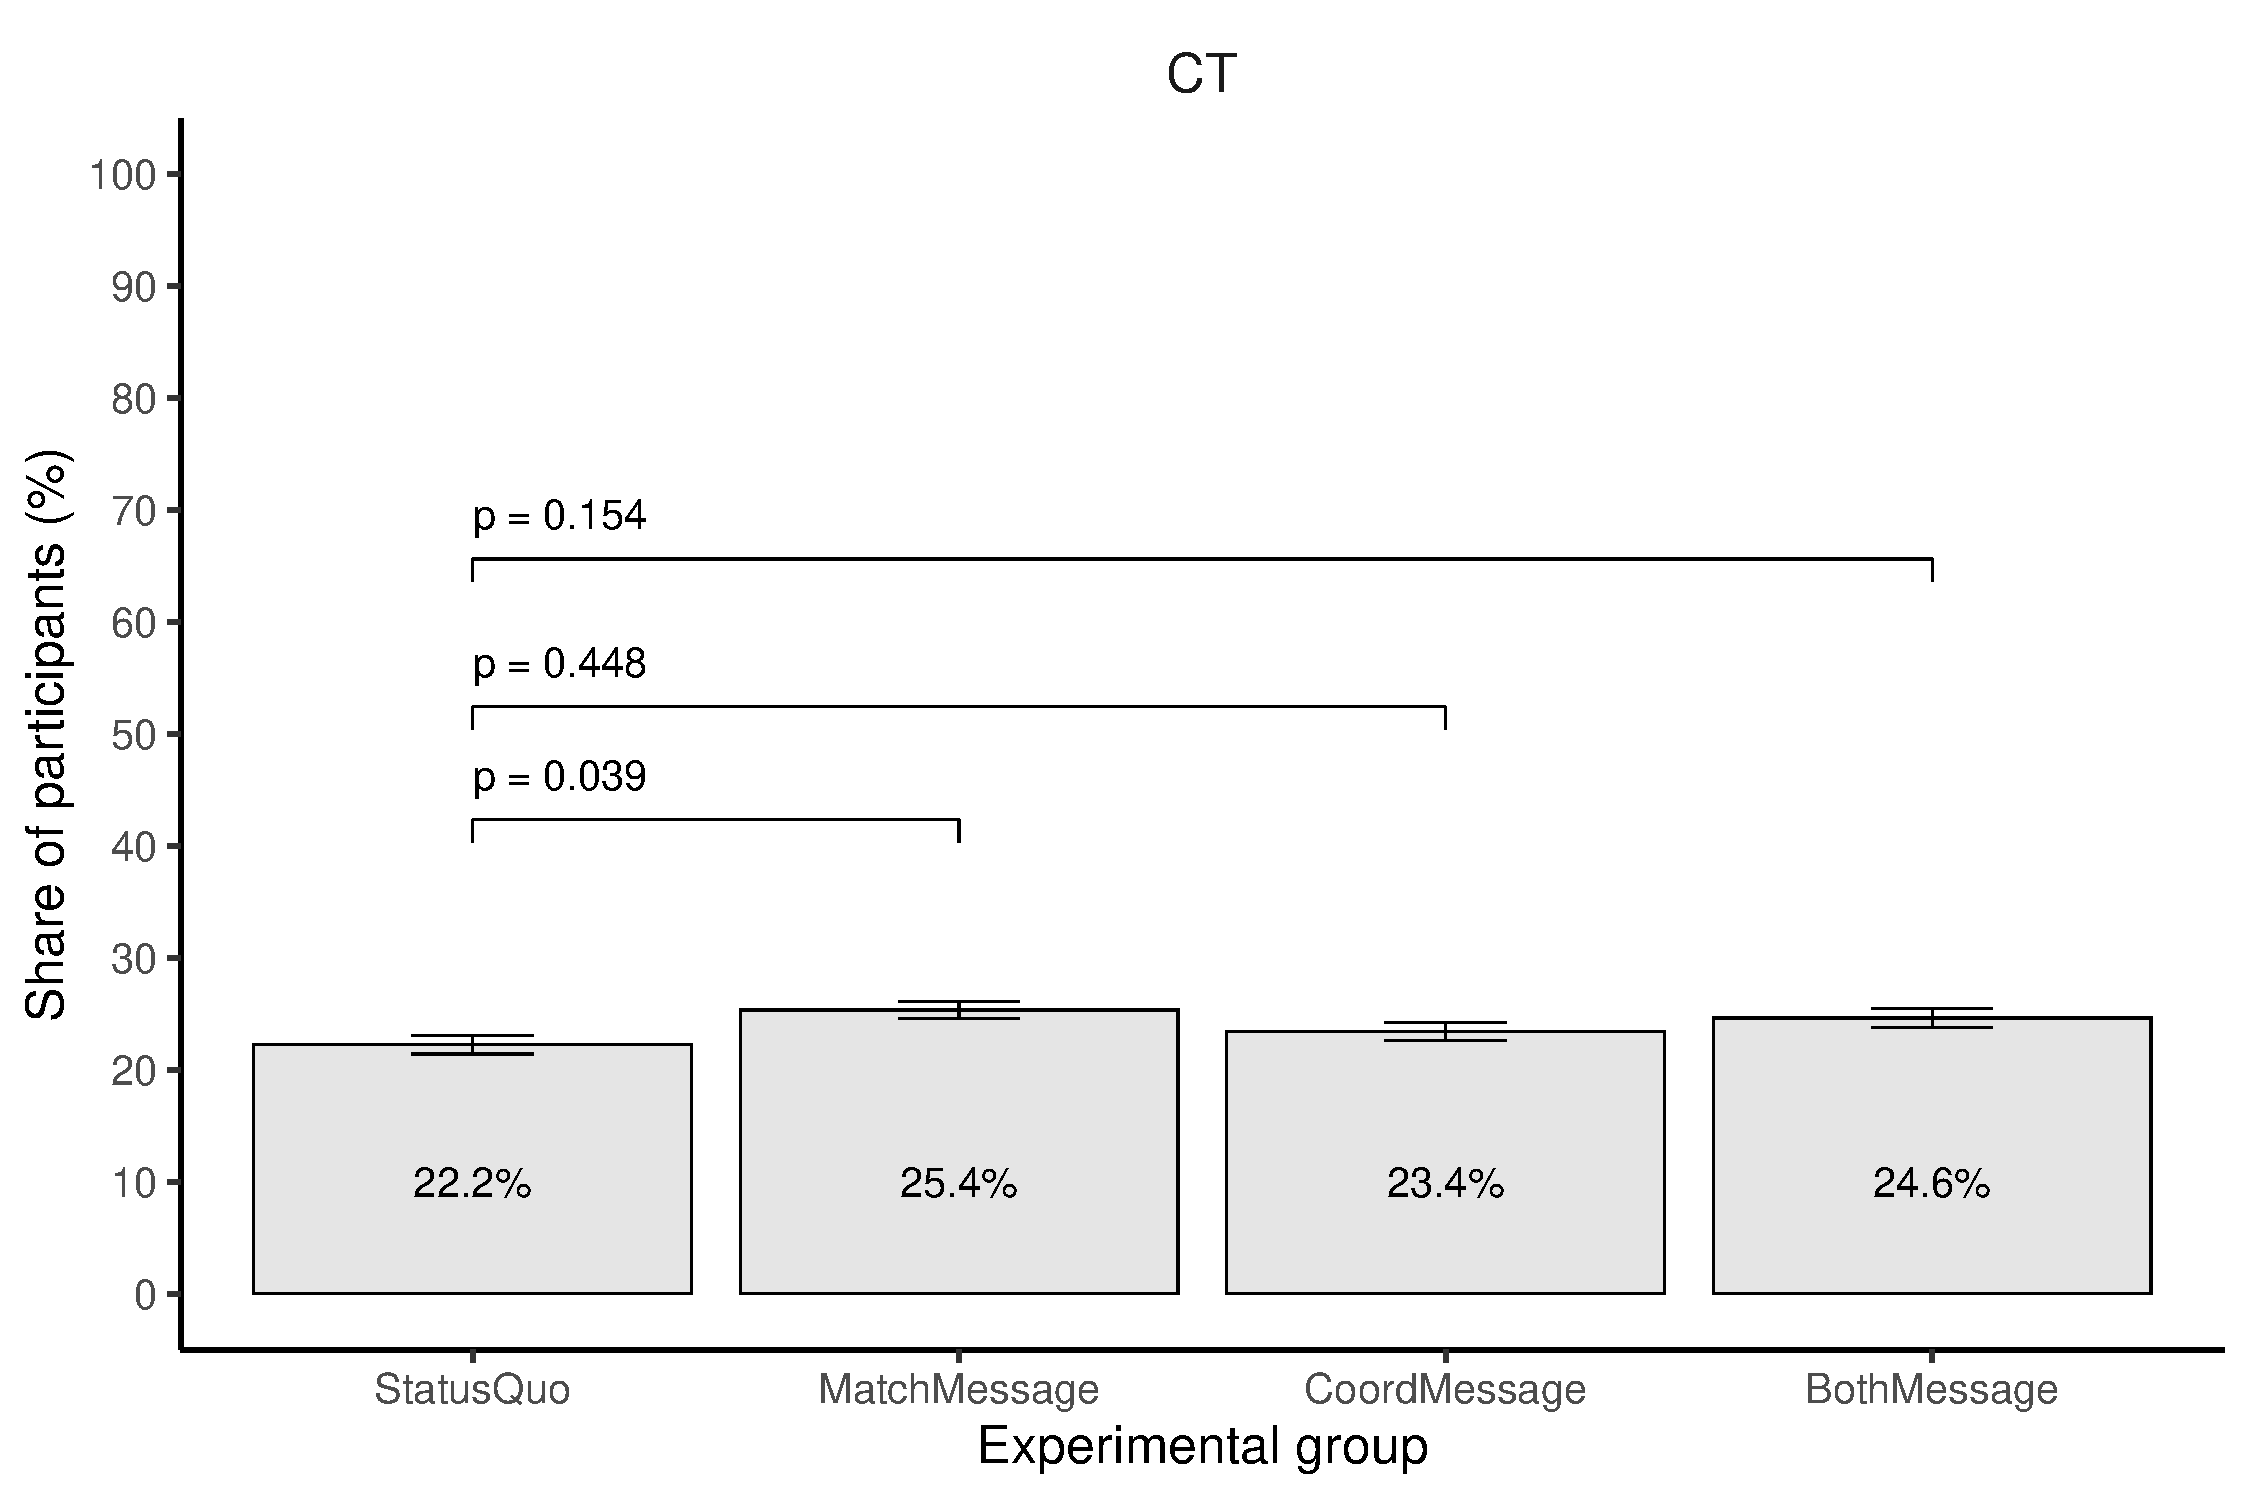
\includegraphics{JMDPRC~2/figure-latex/test-diff-mean-1} \caption{Sample Averages of CT by Treatments.\newline \emph{Note}: Error bars show standard errors of the mean. For the statistical test, we used robust standard errors.}\label{fig:test-diff-mean}
\end{figure}

We show sample averages of each outcome by experimental arms in Figure \ref{fig:stock-diff-mean}. For clarity, the outcomes are arranged from left to right in the order of the coordination process. Figure \ref{fig:stock-diff-mean} shows that experimental arms B and D, which include the probability message, increased the probability of reaching the CT by \(3.1\) and \(2.4\) percentage points, respectively, which is statistically significant. We show the estimation results of the linear probability model in Table \ref{tab:stock-reg}. This suggests that the effects of experimental arms B and D remain robust when controlling for covariates. Moreover, logistic regressions show that 95\% confidence intervals for odds ratios do not include 1 and reject the null hypothesis that no message effects exist (see Table A3 in the Online Supplementary Material A).

Although statistical significance is at the 10\% level, experimental arm B, which includes the probability message, may have increased rates of response with positive intentions by \(2.3\) percentage points, suggesting that the probability message may enhance donor willingness. When controlling for covariates, although statistical significance is at the 10\% level, experimental arm B may have also increased response rates (see Table \ref{tab:stock-reg}). However, logistic regressions showed that 95\% confidence intervals for odds ratios included 1 and failed to reject the null hypothesis that there was no message effect (see Table A3 in the Online Supplementary Material A). Therefore, we cannot robustly obtain the result that the probability message improves donor intentions.

These results suggest that the probability message prevents donor dropout. In the control arm, the attrition rate between responses with positive intentions and the CT is approximately 60\% (\(=1 - 22.2/54.9\)). In contrast, the attrition rate for experimental arms B and D is approximately 56\% (\(=1 - 25.4/57.2\) for experimental arm B). Thus, the probability message, which is included in experimental arms B and D, increases donors reaching the CT stage because these messages help maintain donors' intentions to donate rather than increasing the number of donors willing to donate.

\begin{table}

\caption{\label{tab:stock-reg-subset}Heterogeneous Effects of Message on CT (Age cutoff: 30)}
\centering
\fontsize{9}{11}\selectfont
\begin{threeparttable}
\begin{tabular}[t]{>{\raggedright\arraybackslash}p{3cm}>{\centering\arraybackslash}p{2cm}>{\centering\arraybackslash}p{2cm}>{\centering\arraybackslash}p{2cm}>{\centering\arraybackslash}p{2cm}}
\toprule
\multicolumn{1}{c}{Gender:} & \multicolumn{2}{c}{Female} & \multicolumn{2}{c}{Male} \\
\cmidrule(l{3pt}r{3pt}){1-1} \cmidrule(l{3pt}r{3pt}){2-3} \cmidrule(l{3pt}r{3pt}){4-5}
\multicolumn{1}{c}{Age:} & \multicolumn{1}{c}{$< 30$} & \multicolumn{1}{c}{$30 \le$} & \multicolumn{1}{c}{$< 30$} & \multicolumn{1}{c}{$30 \le$} \\
\cmidrule(l{3pt}r{3pt}){1-1} \cmidrule(l{3pt}r{3pt}){2-2} \cmidrule(l{3pt}r{3pt}){3-3} \cmidrule(l{3pt}r{3pt}){4-4} \cmidrule(l{3pt}r{3pt}){5-5}
  & (1) & (2) & (3) & (4)\\
\midrule
Treatment B & \num{3.24} & \num{1.86} & \num{6.62}** & \num{2.57}\\
 & (\num{3.63}) & (\num{2.08}) & (\num{3.17}) & (\num{1.71})\\
Treatment C & \num{3.97} & \num{0.15} & \num{-0.97} & \num{1.52}\\
 & (\num{3.66}) & (\num{2.19}) & (\num{3.07}) & (\num{1.79})\\
Treatment D & \num{5.70} & \num{4.68}** & \num{-2.49} & \num{2.12}\\
 & (\num{3.61}) & (\num{2.20}) & (\num{3.05}) & (\num{1.77})\\
\midrule
Control average & 20.80 & 18.89 & 23.27 & 24.18\\
Covariates & X & X & X & X\\
Num.Obs. & \num{1132} & \num{3018} & \num{1566} & \num{5333}\\
\bottomrule
\end{tabular}
\begin{tablenotes}
\item \emph{Note}: * $p < 0.1$, ** $p < 0.05$, *** $p < 0.01$. The robust standard errors are in parentheses. The unit of treatment effect is a percentage point. The age category is defined as under 30 years old or older. We controlled for the number of past coordinations, the number of hospitals per 10 square kilometers, the number of hospitals with PBSC collection per 10 square kilometers, the number of hospitals with BM collection per 10 square kilometers, month dummies, and week dummies.
\end{tablenotes}
\end{threeparttable}
\end{table}

The most important intervention is the one that changes the behavior of young males, who have good transplant outcomes but are prone to interrupting coordination. However, the probability message that increases the probability of reaching the CT may negatively impact the probability that young males reach the CT. Conversely, even if the probability message is most effective in young males, it may have negative impacts on other genders and age groups. Therefore, a policy that uniformly assigns the probability message regardless of gender and age may be problematic. An analysis using only the full sample cannot address this point. Therefore, we divided the sample into four subsets by gender and age (under 30 or not) and estimated the message effects in each subset.

The estimation results are presented in Table \ref{tab:stock-reg-subset}. Before discussing the message effects, we noted two important findings regarding the coordination process of young males. First, compared to other gender and age groups, young males had a lower willingness to donate. In the control arm, the response rate for the young male group was \(74.2\)\%, with only \(51.9\)\% (\(=38.5/74.24\)) expressing a willingness to donate. By contrast, response rates for other groups excluding young males exceeded 85\%, with more than 60\% of responses expressing a willingness to donate.\footnote{For females in their 20s, \(59.1\)\% (\(=50.8/86\)); for females over 30, \(62.2\)\% (\(=58.66/94.32\)); for males over 30, \(66.3\)\% (\(=58.44/88.2\)).} Second, compared to other gender and age groups, the attrition rate of young males between responses with positive intentions and the CT was lower. In the control arm, the attrition rate for the young male group was \(39.6\)\% (\(=1-23.27/38.5\)), while the attrition rates for other groups exceeded 50\%.\footnote{For females in their 20s, \(59.1\)\% (\(=1 - 20.8/50.8\)); for females over 30, \(67.8\)\% (\(=1-18.89/58.66\)); for males over 30, \(58.6\)\% (\(=1-24.18/58.44\)).} Therefore, increasing the willingness of young male donors to donate enhances the opportunity for physicians to select young male donors who have good transplant outcomes.

We found that the probability message had a significant impact on the probability of young male donors reaching the CT stage. Experimental arm B, which includes only the probability message, enhanced the CT reach probability for young males by \(6.6\) percentage points, which is statistically significant. This experimental arm also affected the response behavior of young males. Experimental arm B increased the response rate by \(6.4\) percentage points, which is statistically significant. Moreover, it further boosted the response rate with positive intentions by \(9.2\) percentage points, which is also statistically significant.

These results suggest that the probability message suppresses responses with negative intentions. The probability message elevates the intention rate among young male responders from \(51.9\)\% to \(59.2\)\% (\(=(9.22+38.50)/(6.43+74.24)\)). The probability message resolves the problem that the willingness to donate among young males is relatively low. Additionally, this message slightly reduces the attrition rate between responses with positive intentions and the CT from \(39.6\)\% to \(37.4\)\% (\(=1-(6.62+23.27)/(9.22+38.5)\)). Thus, the probability message increases young male donors reaching the CT stage through the increase in intention rather than the decrease in attrition rate.

For other gender and age groups, excluding young males, experimental arm B, containing only the probability message, had no statistically significant effect on the CT reach probability. Experimental arm D, containing both the probability message and the early coordination message, enhanced the CT reach probability for older female groups while having no statistically significant effect on the CT reach probability for other gender and age groups, including young males. Considering these results, the probability message enhances young male donors with favorable transplantation outcomes to reach the CT stage without negatively impacting other groups. Presenting both the probability message and the early coordination message increases older female donors who reach the CT stage without negatively affecting other groups. Therefore, it can be concluded that there is no downside to uniformly assigning only the probability message.\footnote{Table A4 in the Online Supplementary Material A presents the subsample analysis with an age cutoff set at 40. The effect of the probability message (experimental arm B) on young males slightly weakened, while it slightly strengthened for older males. This suggests that in males, the effect of the probability message seems to follow a convex function of age. However, there is no change in our overall conclusion.}

\hypertarget{reply-speed}{%
\subsection{Response Speed to Notification}\label{reply-speed}}

The early coordination message stated that early coordination increases the patient's transplantation rate. Therefore, this message may encourage early responses to the HLA match letter. As the letter recommends responding within 7 days, we define ``early response'' as responding within 7 days. To verify whether the intervention messages increase this early response, we estimated the change of intervention effects over time, using dummy variables indicating response by a certain day as the outcomes. We expect that the early coordination message will promote responses within 7 days.

Figure A1 in the Online Supplementary Material A shows the cumulative response rate up to 40 days after the letter was sent. In the 5--10 days after the letter was sent, the cumulative response rate for all treatment groups was slightly lower than the control arm, which is statistically significant (see Figure A2 in the Online Supplementary Material A). Subsequently, the cumulative response rate for treatment groups B (dashed line) and D (dotted line) was slightly higher than the control arm, which is statistically insignificant for most periods, except for some. Therefore, the early coordination message does not increase the overall response speed.

Given that the effect on responses is heterogeneous by gender and age, as shown in the previous results, we also split the subsample by gender and age and focused on the heterogeneity of the effect on quick responses. Figure A3 in the Online Supplementary Material A shows the cumulative response rate by gender and age groups (age cutoff is 30).

\begin{figure}[t]
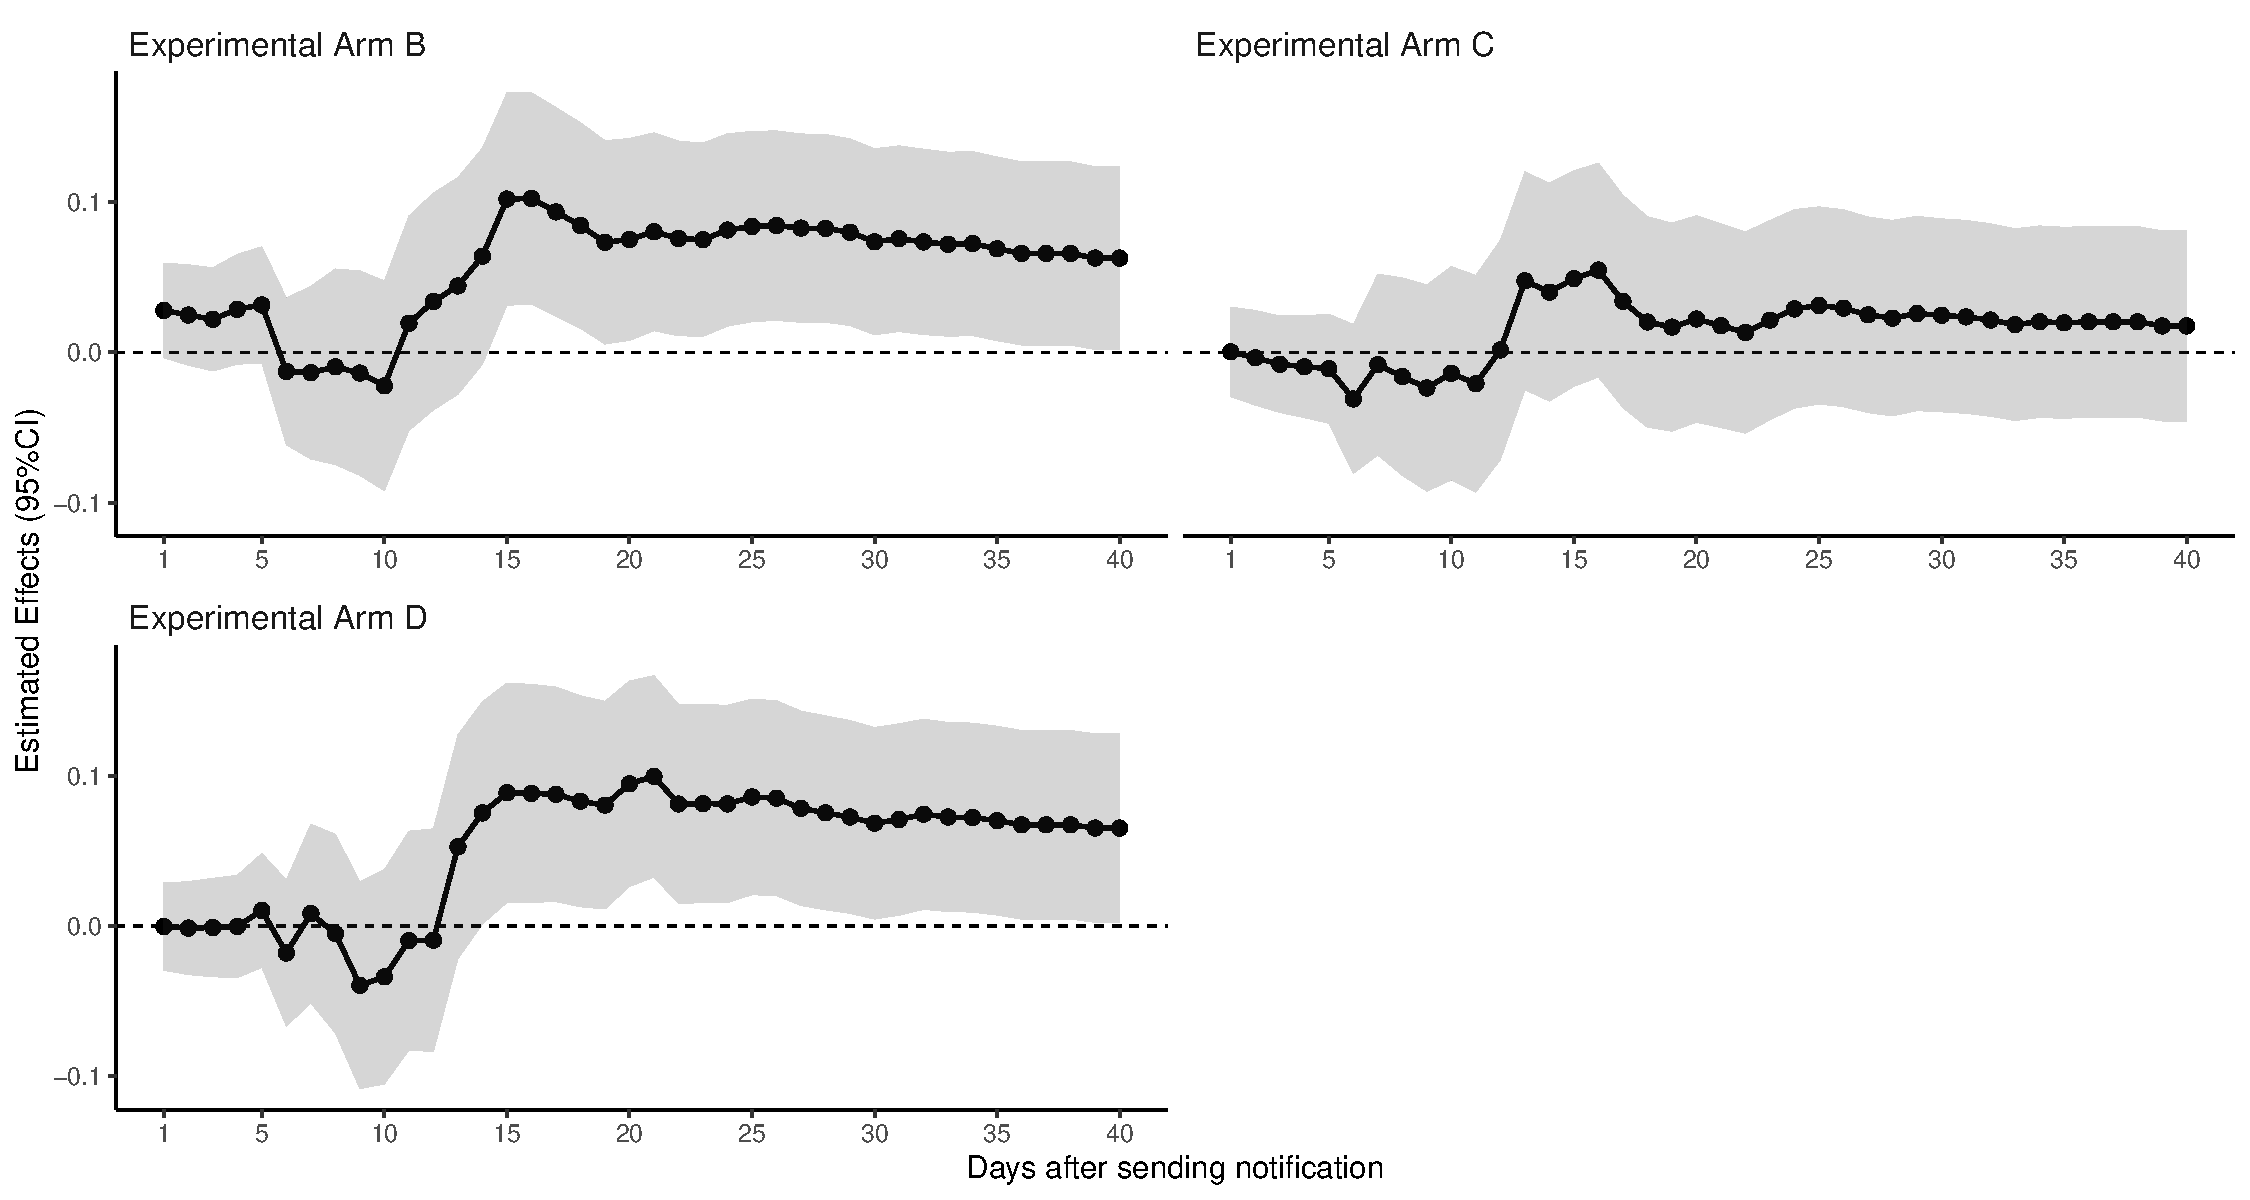
\includegraphics{JMDPRC~2/figure-latex/young-male-flow-1} \caption{Effect on Response Speed of Young Males.\newline \emph{Note}: These plots show the difference in cumulative responses on a specific day between the treated and the control arm (and the associated 95 percent confidential interval). The unit of the treatment effect is a percentage point. We used males younger than 30 for the analysis sample. Further, we used robust standard errors. We controlled for the number of past coordinations, the number of hospitals per 10 square kilometers, the number of hospitals with PBSC collection per 10 square kilometers, the number of hospitals with BM collection per 10 square kilometers, month dummies, and week dummies.}\label{fig:young-male-flow}
\end{figure}

While no significant differences were observed in the pattern of cumulative response rates for males and females aged 30 and older, some notable results were evident for males and females under 30.\footnote{For males and females aged 30 and older, the cumulative response rate for each day differed little between the experimental arms, except for certain periods, and is not statistically significant. See Figure A4 and A5 in Online Supplementary Material A.} In the group of males in their 20s, 15 days after the letter was sent, the responses of experimental arms B and D began to increase relative to those of the controls. Consequently, the cumulative response rate of the two experimental arms is statistically significantly higher than that of the control arm (see Figure \ref{fig:young-male-flow}).\footnote{In the regression analysis, we created a dummy variable that takes 1 if the potential donor responded within \(d\) days as the outcome variable. If the potential donor responded after \(d\) days or did not respond, the outcome variable was 0.} Thus, although experimental arms B and D increased the ultimate response rate among males in their 20s, they did not encourage early responses. This result is natural because the probability message is not intended to encourage early responses. In addition, the trend in experimental arm C, where only the early coordination message was added, was almost the same as that in the control arm; hence, it cannot be said that the early coordination message encourages early responses in this group.

\begin{figure}[t]
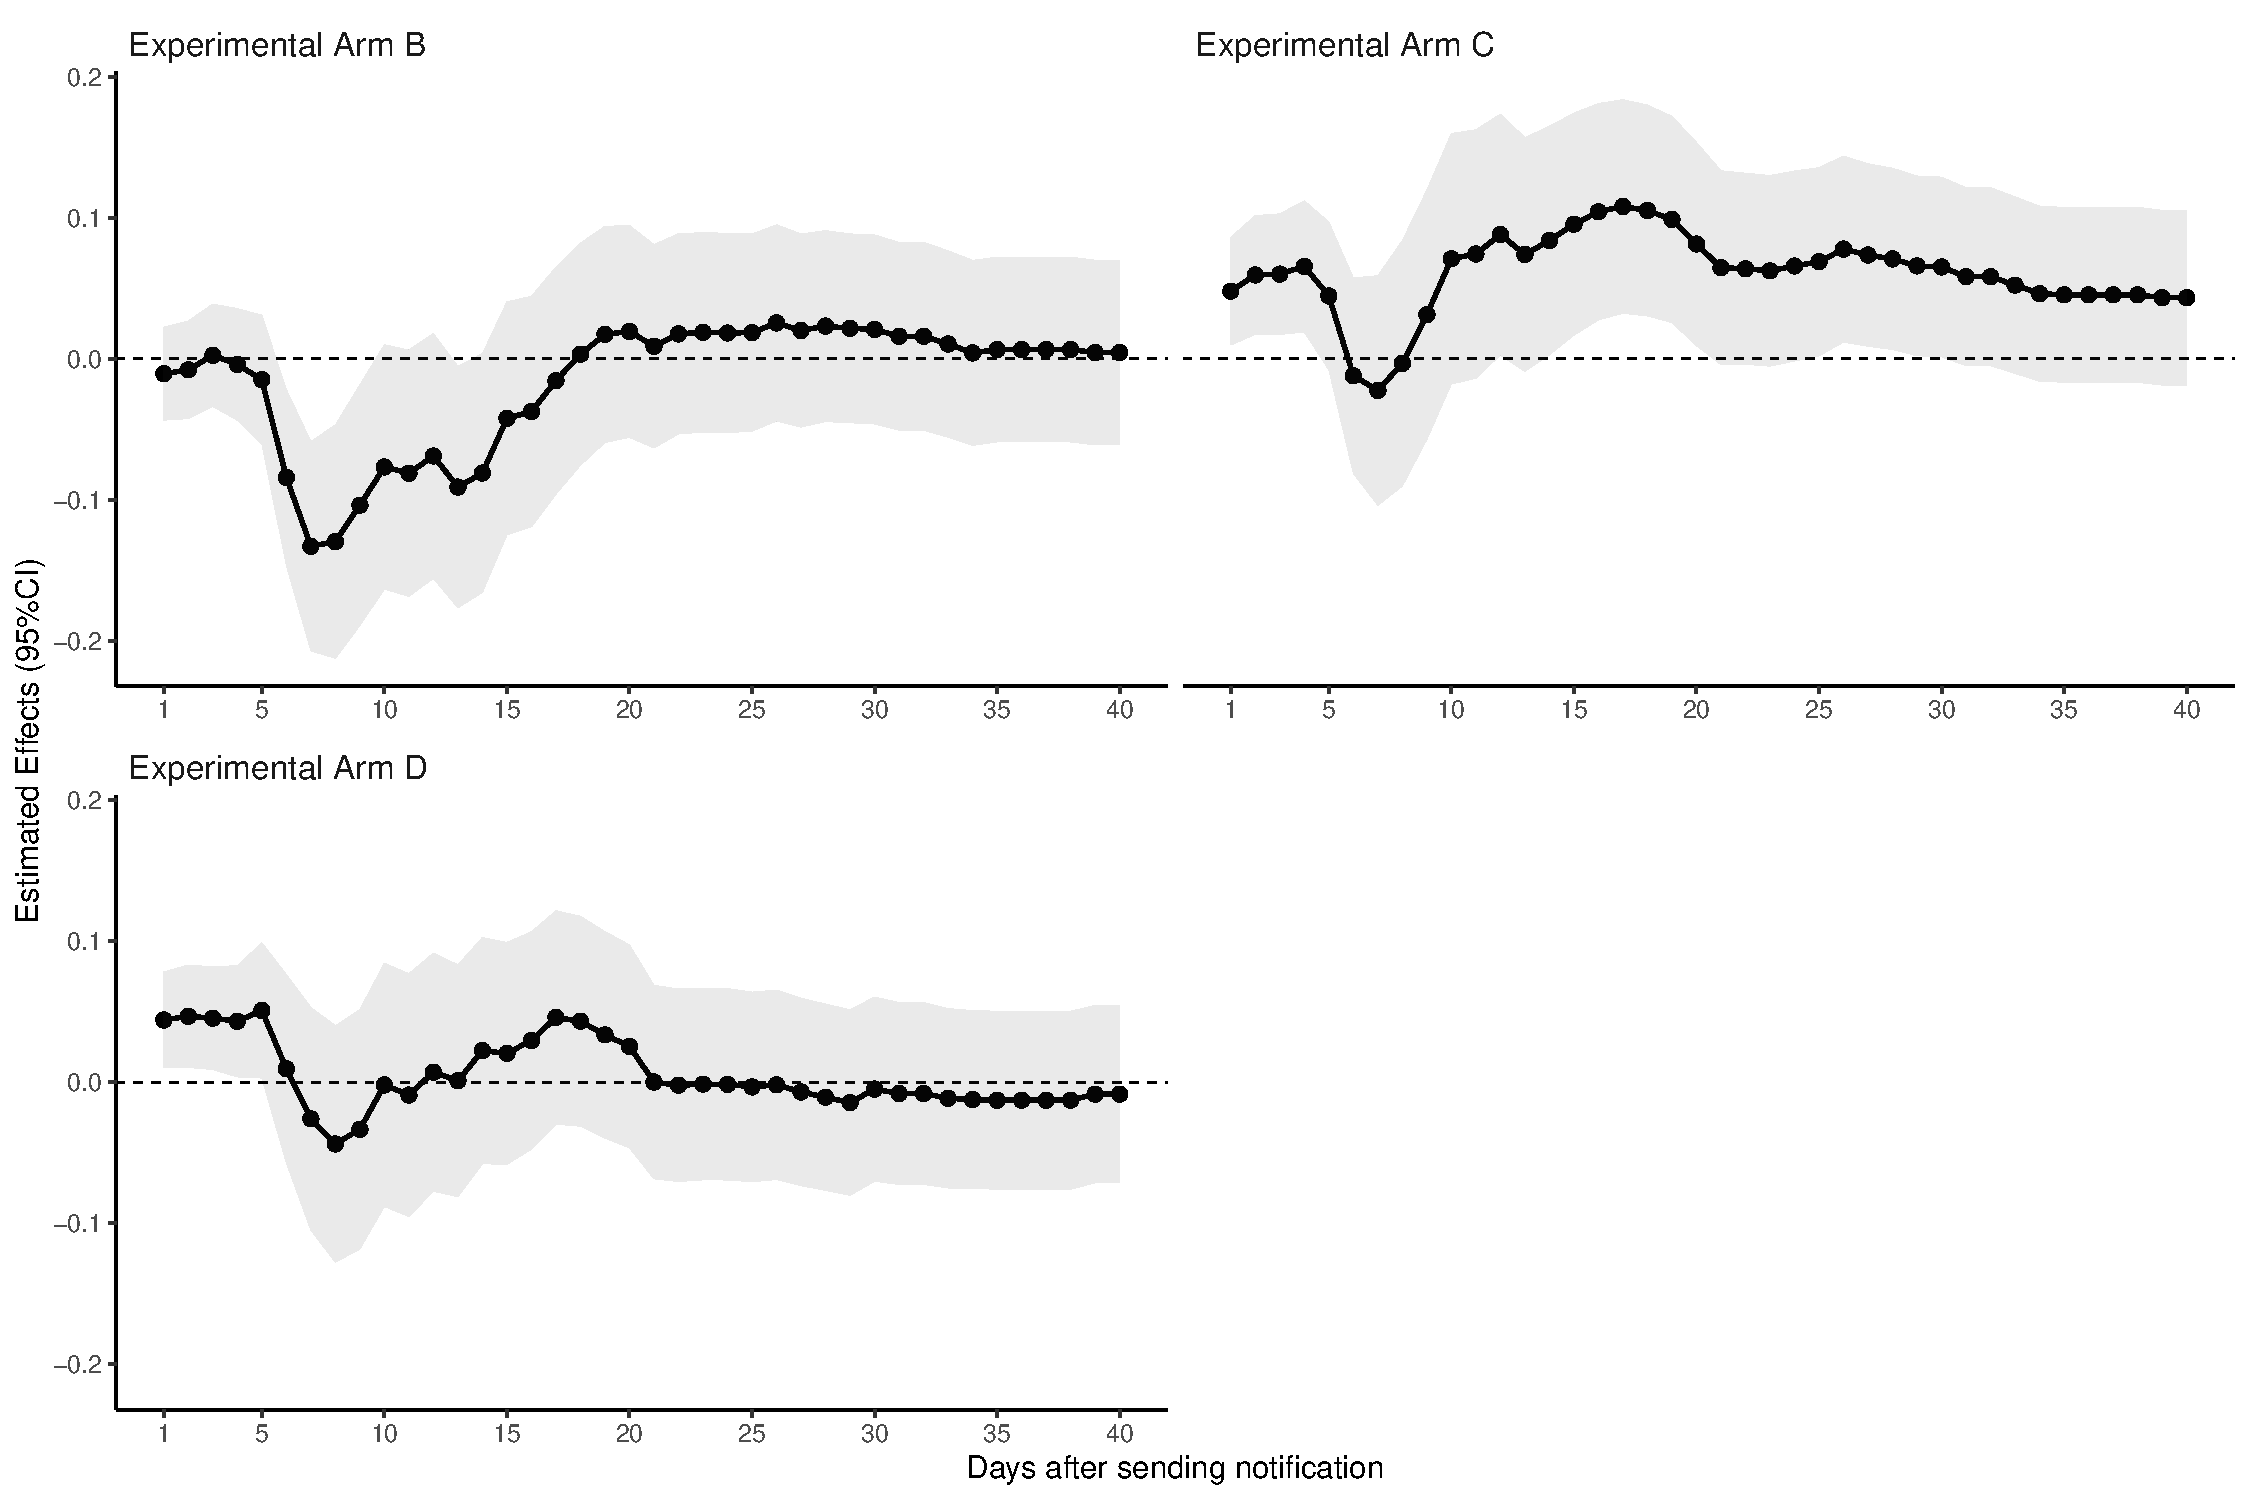
\includegraphics{JMDPRC~2/figure-latex/young-female-flow-1} \caption{Effect on Response Speed of Young Females.\newline \emph{Note}: These plots show the difference in cumulative responses on a specific day between the treated and the control arm (and the associated 95 percent confidential interval). The unit of treatment effect is a percentage point. We used females younger than 30 for the analysis sample. Additionally, we used robust standard errors. We controlled for the number of past coordinations, the number of hospitals per 10 square kilometers, the number of hospitals with PBSC collection per 10 square kilometers, the number of hospitals with BM collection per 10 square kilometers, month dummies, and week dummies.}\label{fig:young-female-flow}
\end{figure}

Compared with the control arm, the responses of experimental arms C and D increased in the group of females in their 20s, within four days of sending the compatibility message. Consequently, the cumulative response rates of the two experimental arms are statistically significantly higher than those of the control arm (see Figure \ref{fig:young-female-flow}). This result suggests that the early coordination message encourages females in their 20s to respond quickly.\footnote{We decomposed the effect of message C on responses within four days (early responses) into two parts in terms of intentions and found that it increased positive and negative intentions to the same extent.}

\hypertarget{process}{%
\subsection{Effects on the Coordination Process}\label{process}}

Finally, we examined the impact of messages on each step of the coordination process after the CT. As explained in Section \ref{background}, the coordination process comprises three stages: candidate selection, final consent, and collection (donation). For the outcome variable, we used a dummy variable that takes the value of 1 if a matched donor has reached each stage. We examined the influence on the post-candidate selection process, acknowledging the involvement of demand-side effects and emphasizing the need for caution in interpretation. In the control arm, \(6.2\)\% became candidates, and \(4.5\)\% ultimately donated.

\begin{figure}[t]
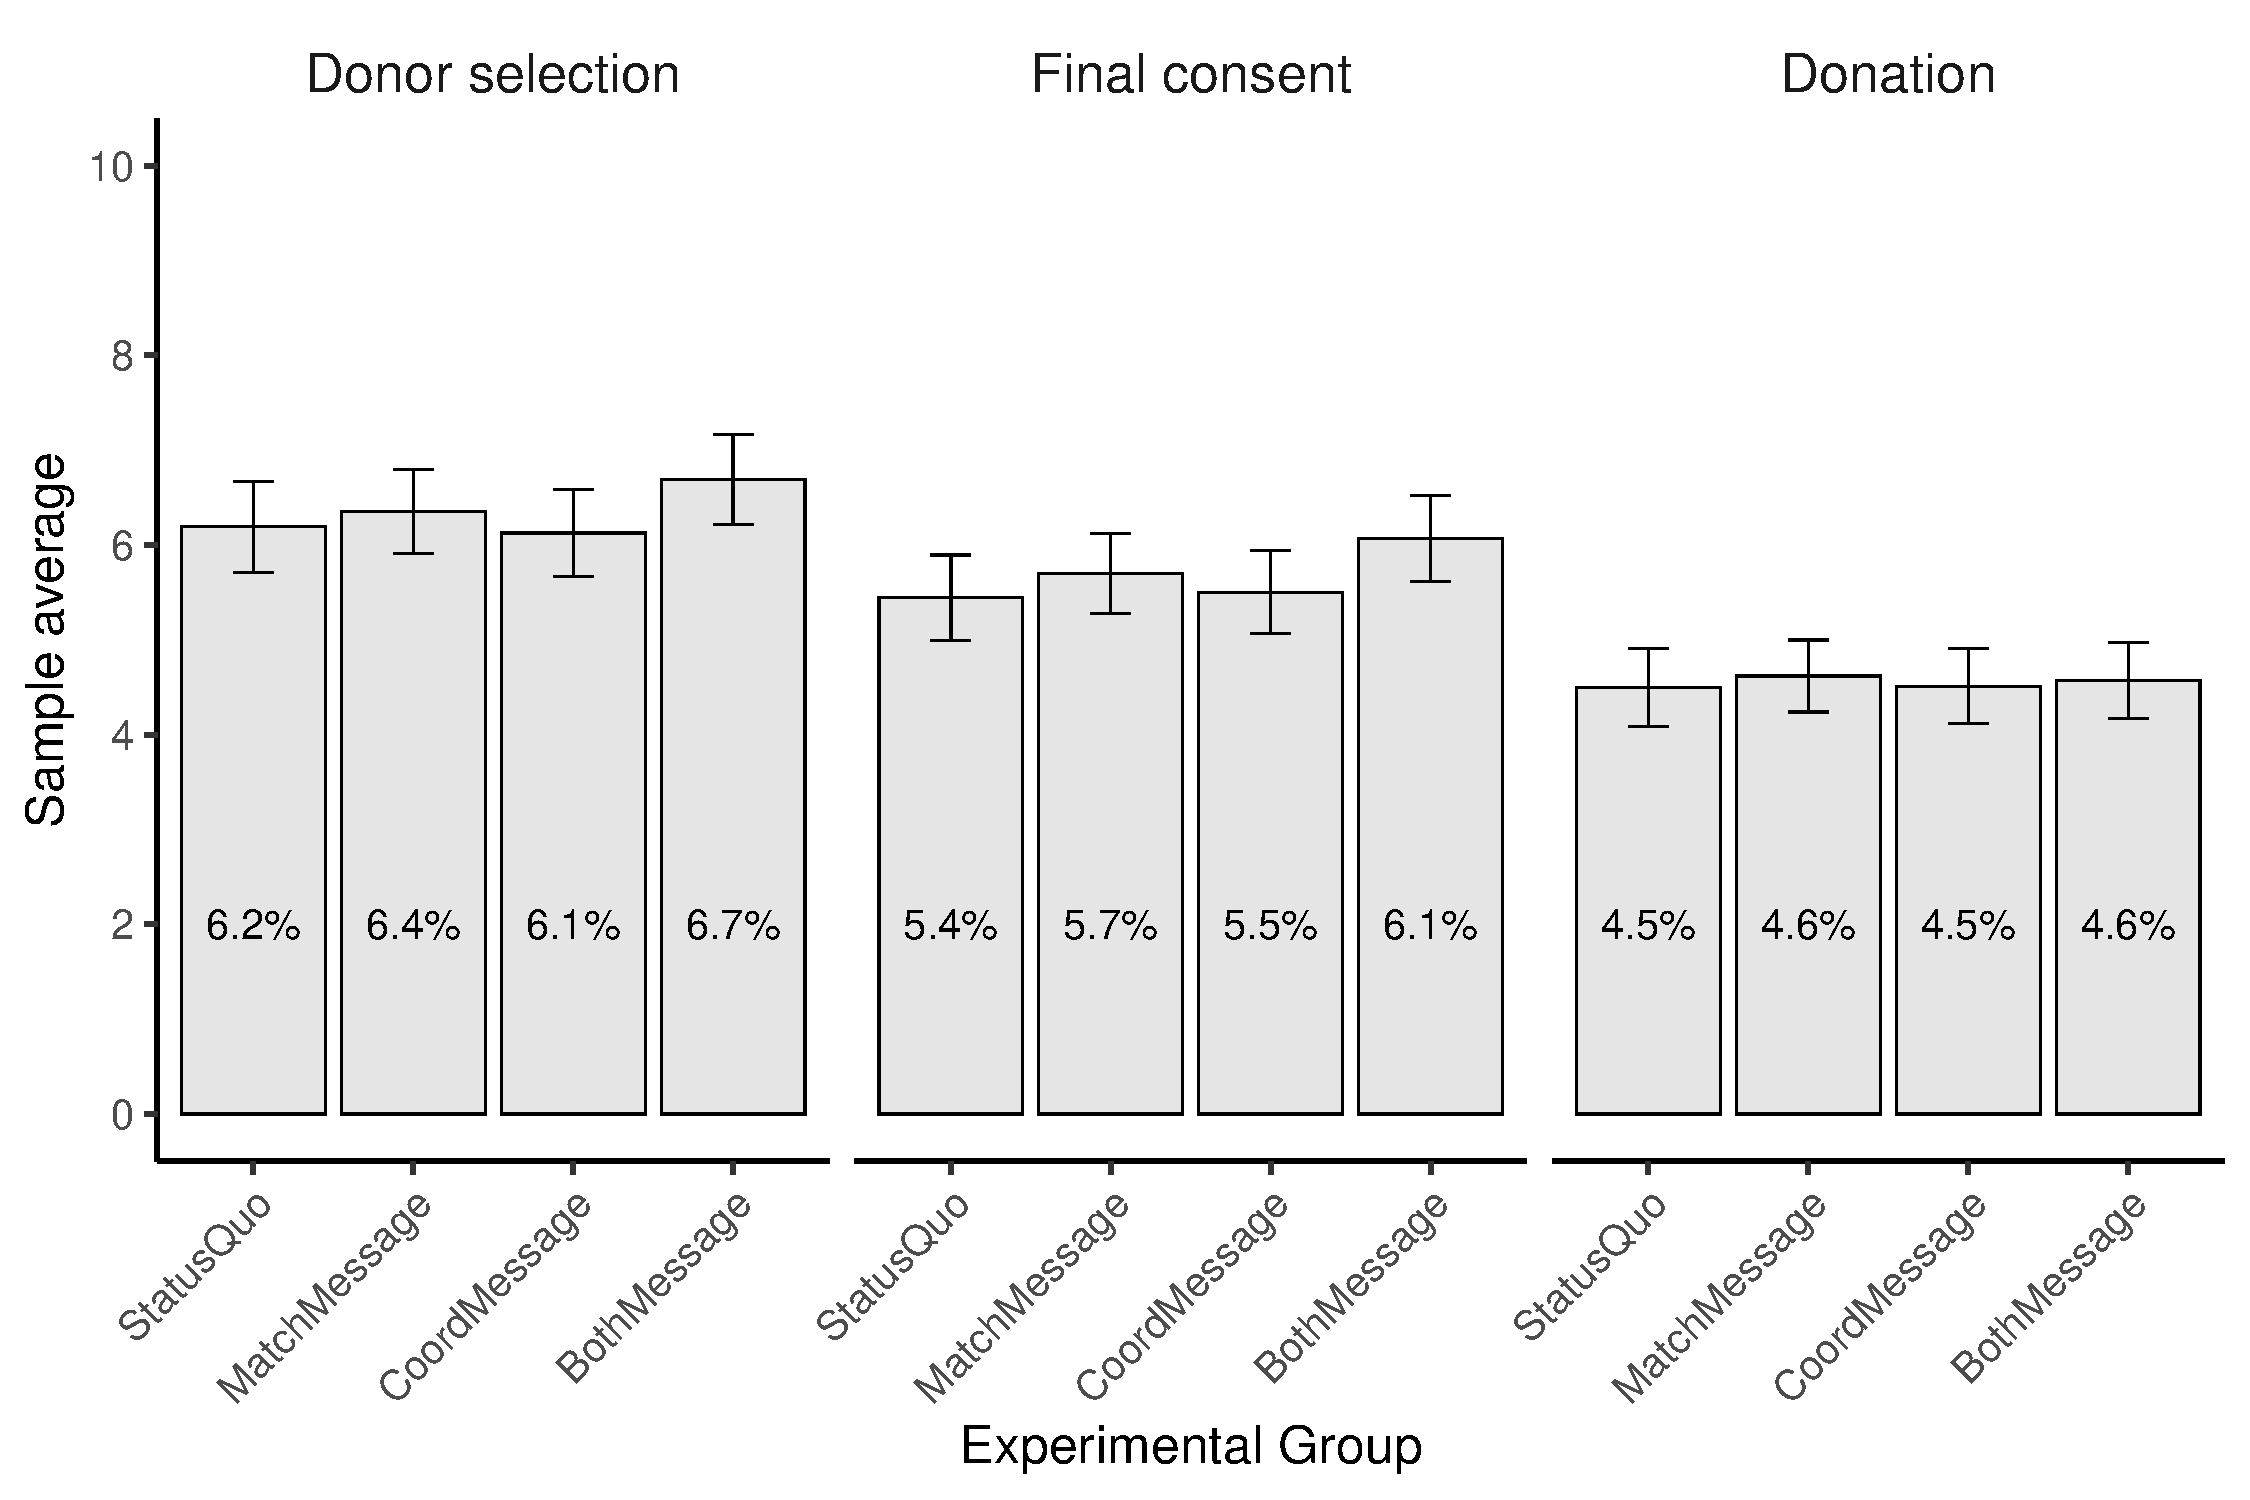
\includegraphics{JMDPRC~2/figure-latex/coordinate-diff-mean-1} \caption{Sample Averages of Candidate Selection, Final Consent, and Donation by Treatments.\newline \emph{Note}: Error bars show standard errors of the mean. For the statistical test, we used robust standard errors.}\label{fig:coordinate-diff-mean}
\end{figure}

We show sample averages of each outcome by treatment in Figure \ref{fig:coordinate-diff-mean}. No experimental arm affected the post-candidate selection process. Similar results were obtained with linear probability models and logistic regressions controlling for covariates (see Table A5 and A6 in Online Supplementary Material A). This result should be interpreted with caution. Given that our intervention does not affect demand (number of patients), if our intervention increases the number of people who reach the CT, it should increase the number of people who are not selected as candidates for exogenous reasons. Particularly, compared to the control arm, experimental arm B increased the probability of donors who reached CT not being selected because of patient-related reasons or donor health conditions by \(4.3\) percentage points. This difference is marginally statistically significant (\(p = 0.095\)). Thus, intervention effects are annulled because of demand-side factors.

\begin{table}

\caption{\label{tab:coordinate-reg-subset}Subsample Analysis for Coordination Process (Age Cutoff: 30)}
\centering
\begin{threeparttable}
\fontsize{9}{11}\selectfont
\begin{tabular}[t]{lccc}
\toprule
 & Candidate selection & Final consent & Donation\\
\midrule
\addlinespace[0.3em]
\multicolumn{4}{l}{\textbf{Young females (N = 1132)}}\\
\hspace{1em}Treatment B & -2.36 (1.96) & -1.69 (1.83) & -0.67 (1.75)\\
\hspace{1em}Treatment C & 0.96 (2.24) & 1.01 (2.07) & 1.41 (1.97)\\
\hspace{1em}Treatment D & -1.47 (2.02) & -1.12 (1.89) & -0.60 (1.74)\\
\hspace{1em}Control average & 6.80 & 5.60 & 4.40\\
\addlinespace[0.3em]
\multicolumn{4}{l}{\textbf{Older females (N = 3018)}}\\
\hspace{1em}Treatment B & -0.91 (0.92) & -0.73 (0.86) & -0.54 (0.82)\\
\hspace{1em}Treatment C & -0.04 (1.05) & 0.24 (0.99) & -0.30 (0.90)\\
\hspace{1em}Treatment D & 0.56 (1.04) & 0.41 (0.94) & -0.33 (0.84)\\
\hspace{1em}Control average & 3.55 & 2.98 & 2.70\\
\addlinespace[0.3em]
\multicolumn{4}{l}{\textbf{Young males (N = 1566)}}\\
\hspace{1em}Treatment B & 2.30 (2.03) & 1.94 (1.88) & 2.87* (1.74)\\
\hspace{1em}Treatment C & -1.40 (1.92) & -0.73 (1.82) & 0.15 (1.68)\\
\hspace{1em}Treatment D & 0.59 (2.08) & 1.42 (1.97) & 1.41 (1.76)\\
\hspace{1em}Control average & 7.76 & 6.37 & 4.71\\
\addlinespace[0.3em]
\multicolumn{4}{l}{\textbf{Older males (N = 5333)}}\\
\hspace{1em}Treatment B & 0.39 (1.05) & 0.36 (1.01) & -0.49 (0.91)\\
\hspace{1em}Treatment C & -0.19 (1.07) & -0.40 (1.03) & -0.55 (0.94)\\
\hspace{1em}Treatment D & 0.97 (1.10) & 0.92 (1.06) & 0.05 (0.96)\\
\hspace{1em}Control average & 7.13 & 6.56 & 5.49\\
\bottomrule
\end{tabular}
\begin{tablenotes}
\item \emph{Note}: * $p < 0.1$, ** $p < 0.05$, *** $p < 0.01$. The robust standard errors are in parentheses. The unit of treatment effect is a percentage point. The age category is defined as under 30 years old or older. We controlled for the number of past coordinations, the number of hospitals per 10 square kilometers, the number of hospitals with PBSC collection per 10 square kilometers, the number of hospitals with BM collection per 10 square kilometers, month dummies, and week dummies.
\end{tablenotes}
\end{threeparttable}
\end{table}

Table \ref{tab:coordinate-reg-subset} divides the sample into four subsets by gender and age (under 30 or not) and estimates the message effect in each subset. The results show that experimental arm B may have increased donations among males in their 20s by 4 percentage points, which is statistically significant at the 10\% level. However, the effect on candidate selection and final consent is not statistically significant. As noted earlier, this effect may reflect not only the effect of our intervention but also the demand for stem cell transplants. Because younger males have better transplant outcomes, the demand for stem cell transplants may be higher in this generation than in other genders and ages. Indeed, in the control arm, the selection probability of young male donors who reached CT was \(33.3\) (\(=7.76/23.27\)) \%, which was higher than other groups.\footnote{For females in their 20s, \(32.7\) (\(=6.80 / 20.80\)) \%; for females over 30, \(18.8\) (\(=3.55 / 18.89\)) \%; for males over 30, \(29.5\) (\(=7.13/24.18\))\%.} In addition, experimental arm C, which encouraged early responses from females in their 20s, had no statistically significant effect on the post-candidate selection process of females in their 20s.\footnote{Table A7 in the Online Supplementary Material A presents the subsample analysis with an age cutoff set at 40. We confirmed that the results did not change.}

\hypertarget{conclusion}{%
\section{Discussion and Conclusions}\label{conclusion}}

This study examined how information provision increases the number of donors from whom physicians can choose the optimal donor for transplantation. The results indicated that information about a low number of HLA-matched donors per patient (probability message) increased the probability of reaching the CT stage. Furthermore, this information increased the probability of male donors in their 20s, who have better transplant outcomes, reaching the CT stage by increasing their willingness to donate. Thus, information about the HLA matching of other donors would increase the efficiency of coordination in the sense that the probability message increases donors, especially young male donors with good transplant performance, reaching the CT stage.

As stated above, the probability message increased the willingness to donate for males in their 20s, suggesting that young males may engage in free-riding behavior. Conversely, the probability message did not affect the willingness to donate for other genders and age groups, suggesting that donors in their groups may not engage in free-riding behavior. One reason for the heterogeneity of the results may be that the altruistic preferences of males in their 20s differ from those of other genders and age groups. Economic studies have suggested that there are two main types of motives for altruistic behavior: warm glow, in which one gains utility from one's altruistic behavior; and pure altruism, in which one gains utility from the results of altruistic behavior, such as the production of public goods \citep[e.g.,][]{Andreoni1990}. Those with a relatively stronger warm glow are less likely to engage in free-riding behavior because they are less concerned about the actions of others. Thus, others may have a stronger warm glow preference than males in their 20s as the main driver of altruistic behavior.

The early coordination message did not affect the overall response rate among females in their 20s; however, it had a positive effect on shorter responses (4 days or less).\footnote{No message encouraged young female donors to donate and reach the CT stage. Given that gender mismatch between donors and patients has increased the risk of GVHD \citep{Loren2006, Nannya2011}, it will be necessary to develop effective informational resources for female donors in future studies.} This suggests that the timing of replies was shortened instead of encouraging response behavior itself. The lack of effects for other genders and ages may be due to the possibility that they already have this information. Alternatively, females in their 20s may have a stronger degree of present bias and a greater tendency toward delayed behavior than other groups. The heterogeneity of the message effect could be explained by differences in information possession or time preferences.

Although this study identifies the causal effects of information provision through field experiments, it is limited by the fact that the data and experimental design do not allow for the identification of the mechanisms described above. This can be considered in future work; for example, scholars may investigate individuals' economic preferences and beliefs before the intervention. Nonetheless, this study has several practical implications. The findings suggest that information provided to donors by the program office at the time of matching with a patient may promote behavioral changes in a desirable direction. However, as some studies have shown that information provision is ineffective \citep[for example,][]{Switzer2018}, the effectiveness of our information provision protocol should be tested in bone marrow donor programs in other countries.

\clearpage

\appendix

\hypertarget{appendix}{%
\section*{Appendix}\label{appendix}}
\addcontentsline{toc}{section}{Appendix}

\hypertarget{message}{%
\section{Text Messages}\label{message}}

The standard HLA match letter is as follows:

\begin{quote}
We inform you that your HLA type (white blood cell type) matches that of a patient on our registry, and you have been selected as one of our potential donors. We are contacting you to ask if you would like to undergo further testing and interviews in preparation for the donation. Please read the enclosed materials carefully, consider whether coordination is possible, and return the form \emph{within seven days} of receiving this information. {[}Insert intervention messages here{]} If we proceed with the coordination after receiving your return, a coordinator will contact you by phone to discuss the details of your request.
\end{quote}

The two intervention messages were as follows.

\begin{itemize}
\tightlist
\item
  \emph{Probability message}: The number of registered donors whose HLA type matches that of a single registered patient is one in hundreds to tens of thousands. We hope you understand that while we may find more than one potential donor, it is not a large number.
\item
  \emph{Early coordination message}: Approximately 60\% of patients can receive a transplant through the JMDP. The earlier a donor can be found to donate bone marrow, the higher that percentage can be.
\end{itemize}

\clearpage

\bibliography{biblio.bib}



\end{document}
